Come si è detto nella sezione dedicata al contesto meteo (par.\ref{cap:meteo}, pag.\pageref{cap:meteo} e sgg.), l'aumento della ventilazione verificatosi in corrispondenza dell'entrata in vigore delle misure di distanziamento e di limitazione della mobilità può costituire un elemento confondente nell'individuazione degli effetti sulla qualità dell'aria del \textit{lockdown}. 

Un modo per aggirare questa interferenza è analizzare i rapporti tra concentrazioni di inquinanti. Infatti i fattori meteo che determinano dispersione degli inquinanti, quali la turbolenza e la ventosità, e quelli che ne determinano l'accumulo agiscono per lo più in maniera ``aspecifica'', cioè senza distinguere tra inquinanti. 
Perciò in prima approssimazione ci si può aspettare che il rapporto tra le concentrazioni di alcuni inquinanti resti sostanzialmente inalterato a prescindere dalla meteorologia.
Dunque l'analisi dei rapporti tra concentrazioni di inquinanti consente di ridurre l'effetto confondente della meteorologia, focalizzandosi meglio sugli effetti delle variazioni delle emissioni.

\FloatBarrier\paragraph{Toluene/benzene}\label{cap:tb}
Il rapporto tra le concentrazioni dei composti organici toluene e benzene è comunemente utilizzato come indicatore della prossimità ad alcune sorgenti emissive. In generale, le emissioni da traffico veicolare, attività industriali e uso di solventi determinano valori del rapporto toluene/benzene superiori ad 1, mentre le emissioni da combustione di biomassa, biocombustibili e carbone determinano valori inferiori a 1 \cite{zhang2016spatiotemporal,seco2013volatile}. 

Dunque l'analisi di questo rapporto prima e durante l'attuazione delle azioni di limitazione alla mobilità individuale, e in particolare il confronto con gli anni precedenti e tra stazioni collocate a distanze diverse dalle strade, può consentire di individuare gli effetti del \textit{lockdown} sulle concentrazioni di composti organici in aria ambiente.

Prima dell'entrata in vigore delle misure di contenimento il rapporto toluene/benzene presentava valori generalmente compresi tra 1 e 2, mentre durante il \textit{lockdown} tale rapporto, pur con alcune fluttuazioni, ha spesso raggiunto valori di 0.5 o anche inferiori (fig.\ref{fig:tbandamento}). Questa evidente variazione può essere in parte attribuita alla netta diminuzione dei flussi di traffico veicolare, in parte ad un probabile lieve aumento delle emissioni da combustione di biomassa per riscaldamento domestico. Temporanei aumenti del consumo di legna per il riscaldamento domestico sono probabilmente la causa delle analoghe diminuzioni del rapporto toluene/benzene osservate occasionalmente negli anni precedenti, durante settimane caratterizzate da temperature particolarmente rigide.

La figura \ref{fig:tbgiorni} riporta i giorni tipo del rapporto toluene/benzene calcolati su periodi di tre settimane ciascuno. Questa suddivisione consente di analizzare separatamente periodi abbastanza omogenei per condizioni meteorologiche e per grado di applicazione delle misure di contenimento del contagio. I grafici della prima colonna riportano l’andamento del giorno tipo prima del \textit{lockdown}, la seconda si riferisce al periodo di sola chiusura delle scuole, le successive due colonne riportano gli andamenti durante il blocco, mentre l’ultima è riferita al periodo in cui il blocco viene parzialmente allentato.

Considerando in particolare le stazioni di Udine (CAI e SDN, fig.\ref{fig:tbgiorni}) si osservano, tanto nel terzo quanto nel quarto periodo, apprezzabili differenze con gli anni precedenti. In particolare, nel terzo periodo (14 marzo -- 04 aprile) il rapporto toluene/benzene risulta essere significativamente inferiore rispetto al quadriennio 2016--2019 durante tutto l’arco della giornata. Nel quarto periodo, caratterizzato da una ventilazione che nel complesso risulta comparabile a quella del quinquennio precedente, il rapporto toluene/benzene evidenzia una apprezzabile diminuzione nelle sole ore pomeridiane; il fenomeno può essere spiegato con l’aumento dei livelli di ozono che è stato registrato in quel periodo e alla conseguente diminuzione delle concentrazioni di toluene nell’aria (che viene rimosso tramite reazioni di degradazione ossidativa).
Nel  quinto e ultimo periodo (nel quale lentamente riprendono alcune attività produttive) i giorni tipo si riallineano con gli anni scorsi.


\begin{figure}
    \centering
    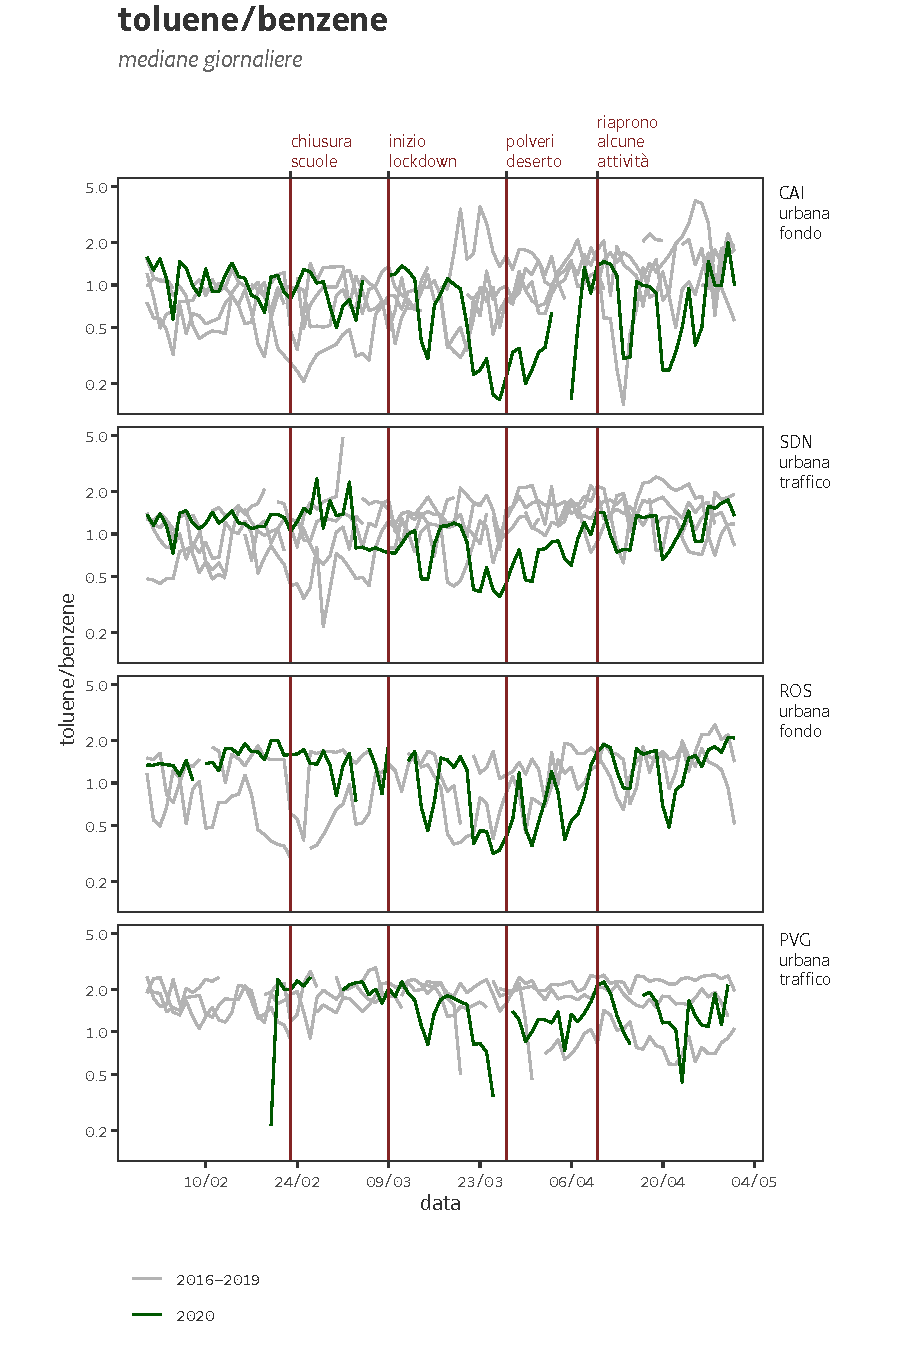
\includegraphics[trim=0 0 0 2cm, clip, width=0.9\textwidth]{{figs/dailyLastVsPast_TB_20200201-20200501}.pdf}
    \caption[Andamento del rapporto toluene/benzene]{Andamento del rapporto toluene/benzene nel periodo febbraio--aprile 2020. Mediane giornaliere confrontate con gli anni precedenti.}
    \label{fig:tbandamento}
\end{figure}

\begin{figure}
    \centering
    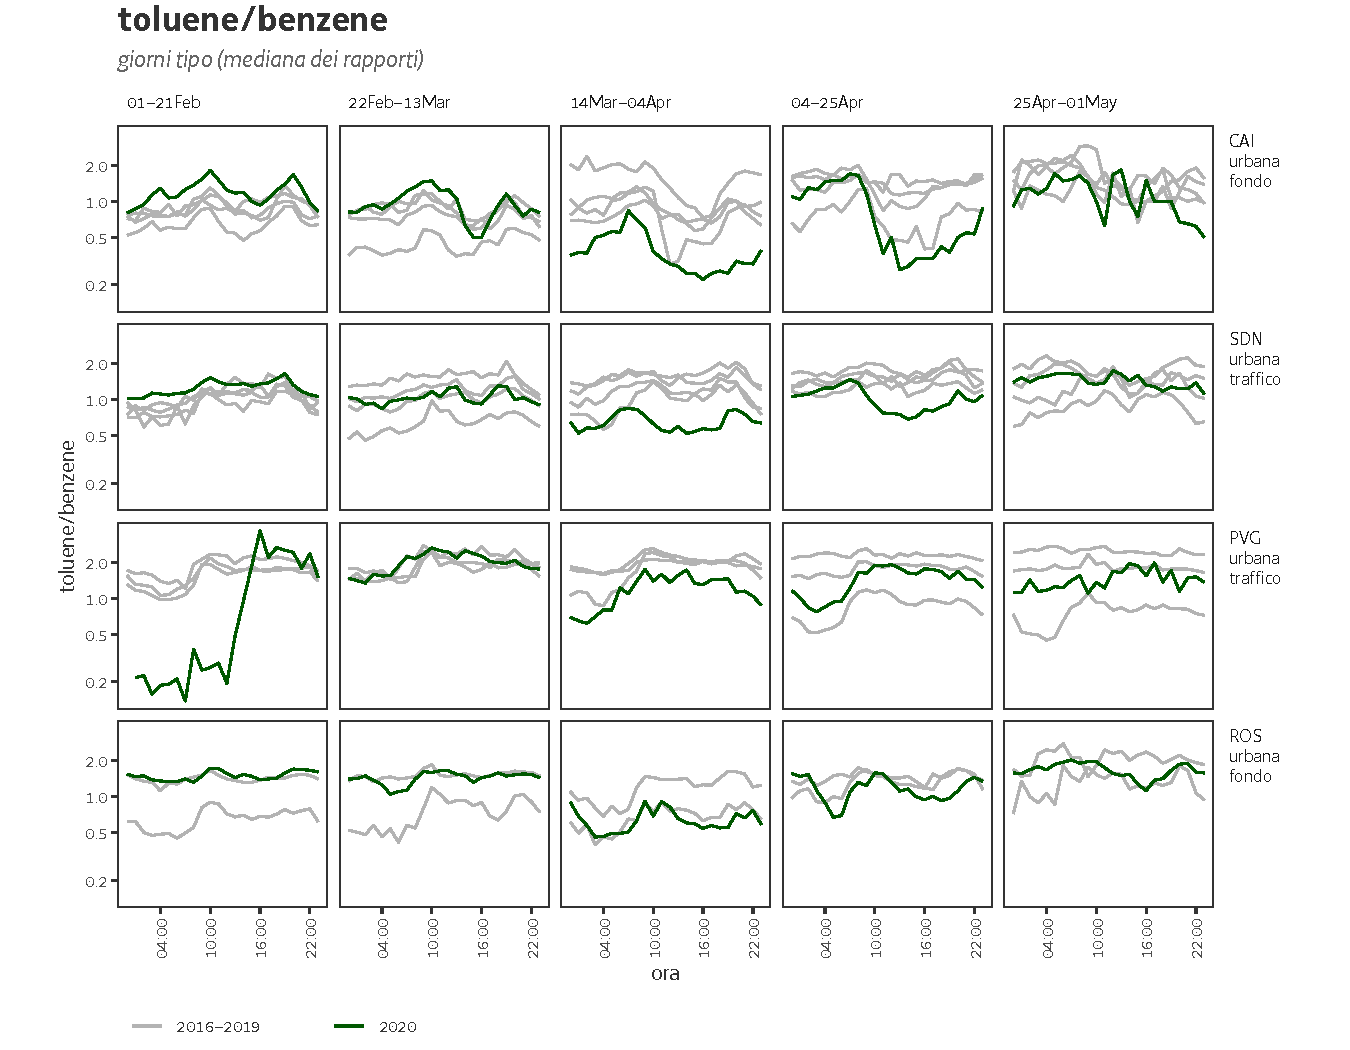
\includegraphics[width=\textwidth]{{figs/medianDay_LastVsPast_TB_20200201-20200501}.pdf}
    \caption[Giorni tipo del rapporto toluene/benzene]{Giorni tipo del rapporto toluene/benzene calcolati ogni tre settimane nel periodo febbraio--aprile 2020, confrontati con gli anni precedenti.}
    \label{fig:tbgiorni}
\end{figure}

%\begin{figure}
%    \centering
%    \includegraphics[width=0.9\textwidth]{{figs/daily_TB_20200201-2020043%0}.pdf}
%    \caption[Rapporto toluene/benzene, confronto tra stazioni]{Andamento del rapporto toluene/benzene nel periodo febbraio--aprile 2020. Mediane giornaliere, confronti tra stazioni della stessa città.}
%    \label{fig:tbconfronti}
%\end{figure}

\FloatBarrier
\paragraph{Ossidi di azoto}\label{cap:noxno}

Fermo restando il ruolo delle condizioni meteo nell’azione di dispersione degli inquinanti atmosferici, il rapporto diagnostico NOx/NO è una grandezza adimensionale il cui valore dipende sia dalla distanza delle fonti emissive di ossidi di azoto sia dai fattori che influenzano la   cinetica chimica dell’ossidazione dell’NO a NOx durante il corso della giornata.

Essendo la specie NO un inquinante primario emesso direttamente dal traffico veicolare, il rapporto NOx/NO viene indagato per poter comprendere se vi siano variazioni peculiari durante il periodo di \textit{lockdown} rispetto agli andamenti degli anni precedenti, considerando sia stazioni da traffico direttamente interessate dal blocco veicolare sia stazioni di fondo per confronto.
In seguito al blocco infatti il flusso di traffico è diminuito drasticamente in regione (fig.\ref{fig:riduzionedeterminanti}) pertanto ci si attende che la riduzione di una fonte importante di NO provochi un aumento contestuale del rapporto diagnostico NOx/NO.

La figura \ref{fig:noxandamento} riporta l’andamento del valore mediano giornaliero del rapporto NOx/NO riferito al periodo febbraio -- aprile 2020 (linea verde) confrontato con i trend misurati per il medesimo periodo negli ultimi 5 anni di monitoraggio (linee grigie).
Osserviamo che le stazioni più suscettibili all’aumento del rapporto NOx/NO sembrano essere quelle da traffico (SDN a Udine, AOS a Gorizia e soprattutto PNC a Pordenone) in cui il blocco ha ridotto sensibilmente le concentrazioni di NO con conseguente aumento  del rapporto diagnostico. Per la stazione da traffico PVG di Trieste il trend è meno evidente.
Le stazioni di fondo (CAI e ROS) mostrano invece un andamento in linea con gli anni precedenti, segno che la riduzione delle emissioni dovuta al \textit{lockdown} ha avuto effetti più marcati in prossimità delle strade.

La figura \ref{fig:noxgiorni} riporta i giorni tipo del rapporto NOx/NO calcolati su periodi di tre settimane ciascuno. Questa suddivisione consente di analizzare separatamente periodi abbastanza omogenei per condizioni meteorologiche e per grado di applicazione delle misure di contenimento del contagio. I grafici della prima colonna riportano l’andamento del giorno tipo prima del \textit{lockdown}, la seconda si riferisce al periodo di sola chiusura delle scuole, le successive due colonne riportano gli andamenti durante il blocco, mentre l’ultima è riferita al periodo in cui il blocco viene parzialmente allentato.

In condizioni normali (prima colonna in fig.\ref{fig:noxgiorni}) il rapporto NOx/NO presenta i valori minimi in corrispondenza dei picchi di traffico, la mattina e la sera, e i valori massimi nelle ore notturne, quando quasi tutto l’NO prodotto nella fase diurna viene ossidato a NOx. Con l'attuazione del blocco (terza e quarta colonna) viene meno il minimo serale e in generale i valori del rapporto NOx/NO aumentano, in alcune stazioni di traffico (Pordenone 14 marzo -- 25 aprile, Gorizia 25 aprile -- 1 maggio) discostandosi dagli andamenti degli anni precedenti. Tuttavia lo scostamento dei giorni medi di NOx/NO rientra nella maggior parte dei casi nell'intervallo di naturale variabilità interannuale.

\begin{figure}
    \centering
    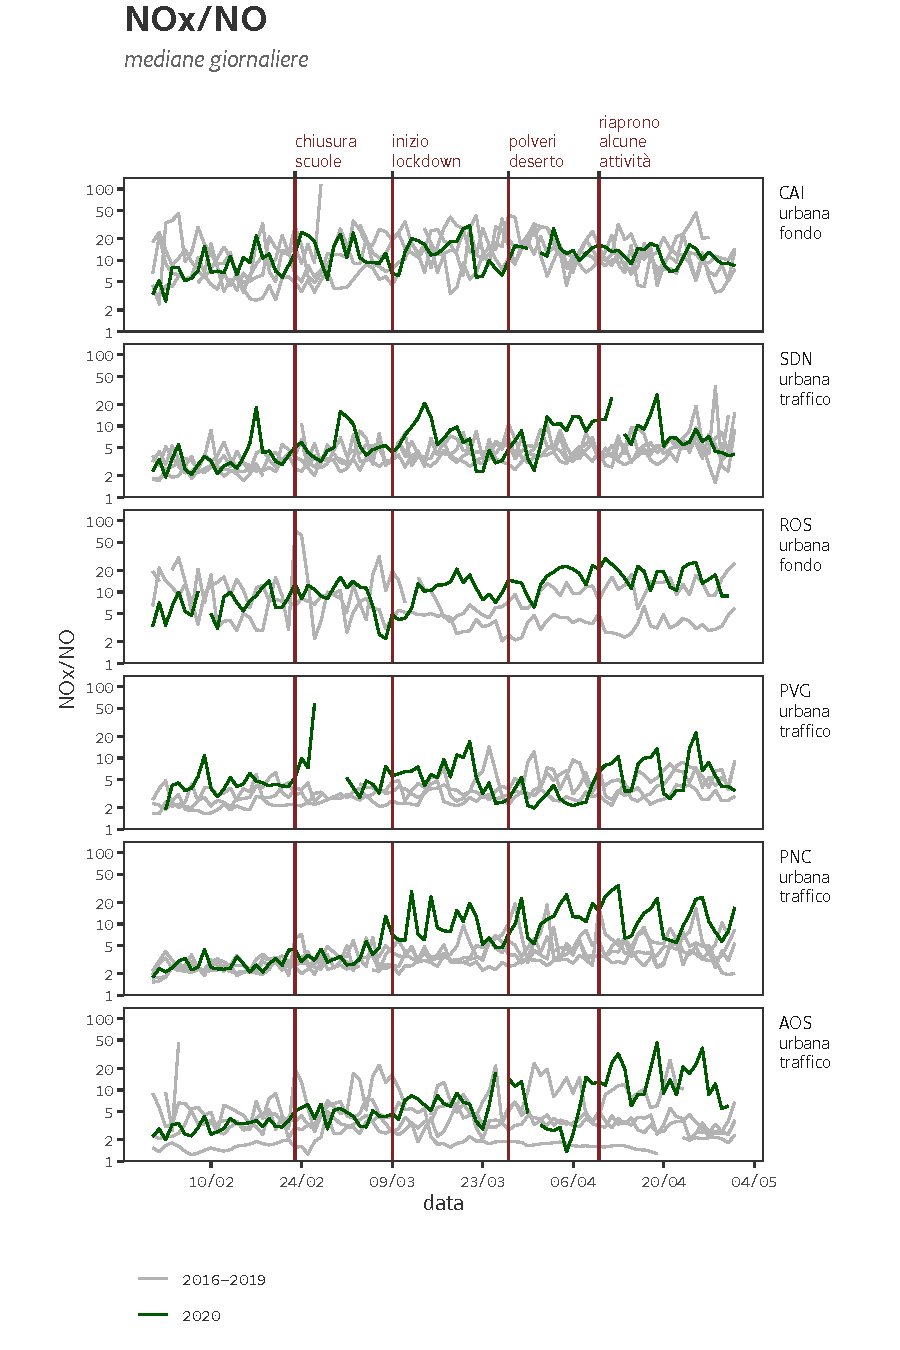
\includegraphics[trim=0 0 0 2cm, clip,width=0.9\textwidth]{{figs/dailyLastVsPast_NOXNO_20200201-20200501}.pdf}
    \caption[Andamento del rapporto NOx/NO]{Andamento del rapporto NOx/NO nel periodo febbraio--aprile 2020. Mediane giornaliere confrontate con gli anni precedenti.}
    \label{fig:noxandamento}
\end{figure}

\begin{figure}
    \centering
    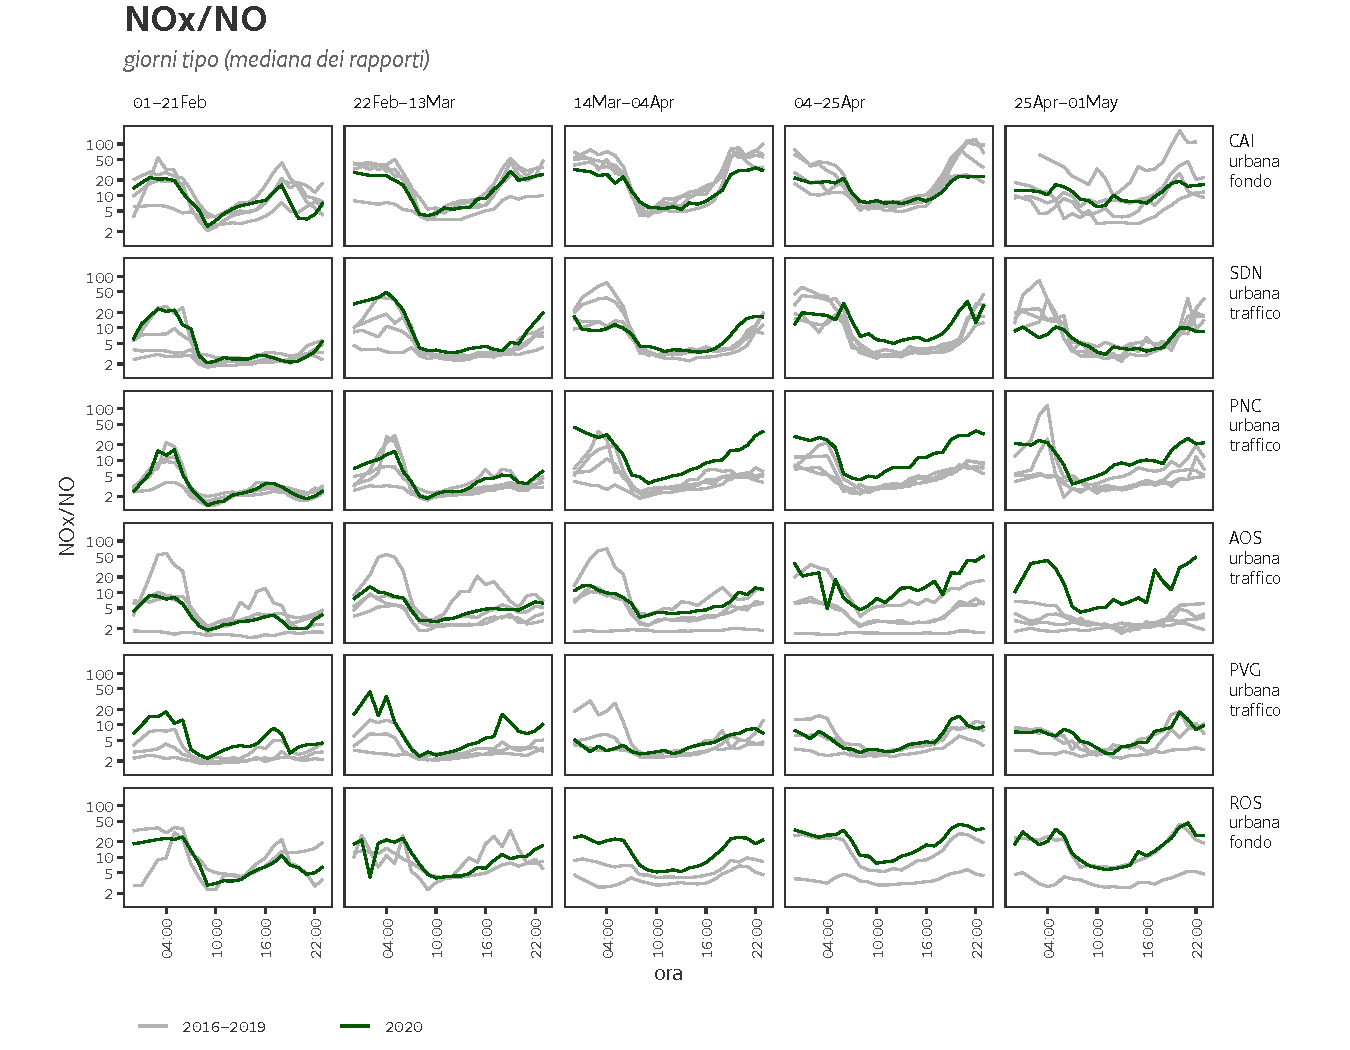
\includegraphics[width=\textwidth]{{figs/medianDay_LastVsPast_NOXNO_20200201-20200501}.pdf}
    \caption[Giorni tipo del rapporto NOx/NO]{Giorni tipo del rapporto NOx/NO calcolati ogni tre settimane nel periodo febbraio--aprile 2020, confrontati con gli anni precedenti.}
    \label{fig:noxgiorni}
\end{figure}

%\begin{figure}
%    \centering
%    \includegraphics[width=0.9\textwidth]{{figs/daily_NOXNO_20200201-2020%0430}.pdf}
%    \caption[Rapporto NOx/NO, confronto tra stazioni]{Andamento del rapporto NOx/NO nel periodo febbraio--aprile 2020. Mediane giornaliere, confronti tra stazioni della stessa città.}
%    \label{fig:noxconfronti}
%\end{figure}

\FloatBarrier
\paragraph{Granulometria delle polveri}\label{cap:cef}

Le frazioni granulometriche usualmente utilizzate per lo studio della formazione del materiale particolato (polveri) in atmosfera sono il PM\textsubscript{10} (polveri con diametro aerodinamico inferiore ai 10~micron), il  PM\textsubscript{2.5} (polveri con diametro aerodinamico inferiore ai 2.5~micron) e il  PM\textsubscript{coarse} ($PM_{10}-PM_{2.5}$, polveri con diametro aerodinamico compreso tra i 2.5 e i 10~micron).

Qui consideriamo il coefficiente di arricchimento percentuale della frazione \textit{coarse} (CEF, \textit{Coarse Enrichment Factor}) 
$$CEF=\frac{(PM_{10}-PM_{2.5})}{PM_{10}} \cdot 100$$

Questo parametro è adimensionale e variabile tra 0 e 100. Esso consente di valutare se l'andamento della frazione grossolana (\textit{coarse}) delle polveri sia correlato alle condizioni meteorologiche e/o alle sorgenti emissive locali.
 Per poter capire meglio gli andamenti e le dinamiche che governano questa grandezza è necessario sempre considerare almeno due punti di misura interessati da sorgenti emissive significativamente diverse (per esempio una stazione di fondo urbano e una stazione da traffico) ma anche spazialmente vicini e dunque soggetti alle stesse condizioni meteo. Così facendo le variabili meteo-climatiche che agiscono sulle due stazioni non rischiano di divenire un fattore confondente per la comprensione degli andamenti del CEF.  
Lo studio in oggetto ha riguardato siti di misura distanti pochi chilometri:  la stazione di Pordenone centro (urbana da traffico) e la stazione di Brugnera (suburbana di fondo).

Il periodo di misura considerato va dal 24/01 al 22/05/2020 comprendente pertanto una fase precedente al \textit{lockdown}, il \textit{lockdown} stesso e una fase successiva al blocco.
Dall'insieme di dati analizzati sono stati esclusi i giorni 27--29 marzo perché disturbati da episodi di ricaduta  di polveri grossolane provenienti dai deserti asiatici.
Inoltre dall'analisi sono escluse le giornate con $PM_{2.5}<7 \mu g/m^3$, cioè con concentrazioni di polveri molto basse.

La figura \ref{fig:cef} riporta gli andamenti medi giornalieri del CEF relativi alla stazione di traffico (Pordenone centro)  e la stazione di fondo suburbano (Brugnera) nel periodo considerato. Entrambe le stazioni sono situate nell'area pordenonese, perciò si possono considerare interessate, in prima approssimazione, dai medesimi determinanti meteo-climatici. 

Si nota un progressivo aumento del CEF nel corso del periodo, in parte attribuibile al graduale venir meno di una rilevante fonte emissiva di particolato fine, la combustione di legna negli impianti di riscaldamento domestici.

Ciò che è interessante rilevare è lo scarto tra la stazione di traffico e la stazione di fondo. Prima del blocco in prossimità delle strade si registra un CEF sistematicamente più alto, cioè un maggior contributo della frazione grossolana, probabilmente determinato dall'azione di risollevamento delle polveri depositate sull'asfalto, causata dal frequente passaggio di veicoli. Durante il \textit{lockdown} invece il CEF nelle due stazioni è molto simile, segno che è venuto meno quel contributo alla concentrazione di polveri sottili, importante ma limitato alle aree più urbanizzate e trafficate.

\begin{figure}
    \centering
    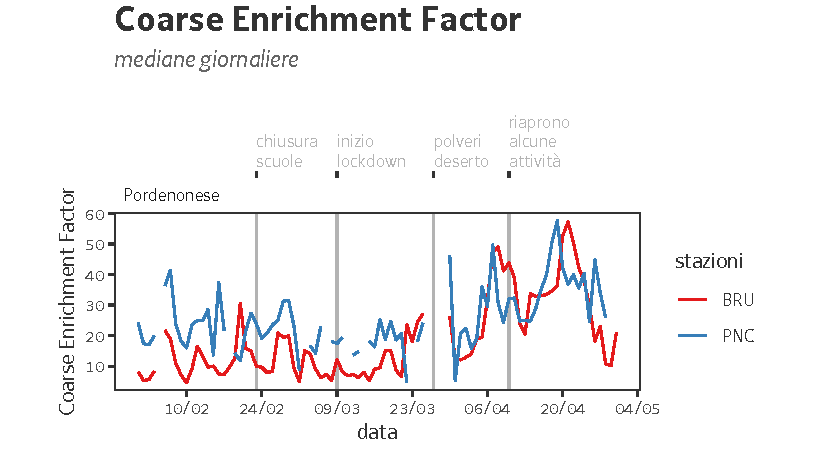
\includegraphics[trim=0 0 0 2cm, clip,width=0.9\textwidth]{{figs/daily_CEF_20200201-20200430}.pdf}
    \caption[Percentuale di polveri grossolane nel PM10, confronto tra stazioni]{Andamento della percentuale di polveri grossolane nel PM10 nel periodo febbraio--aprile 2020. Medie giornaliere, confronti tra stazioni dell'area pordenonese.}
    \label{fig:cef}
\end{figure}
